\section{Theory}

\subsection{Modal Haplotype}

Phyloage uses Y-STR mutation counting to estimate the TMRCA
(Time to Most Recent Common Ancestor) for a group of persons.
This is not an easy task because STR markers jump back and
forth. If a marker has changed from one value to another and
back again we do not know if a mutation has taken place or
not. So for long time spans STR mutation counting does not
work and we get wrong TMRCA estimates. In many cases this
effect can be calculated and compensated as it has been done
in \cite{Kly09}. However this method has it's limits.

Phyloage uses another approach. It combines SNP based phylogenetic
trees and Y-STR counting. Because of the use of SNPs, the
ancestral positions on the phylogenetic tree are well known.
Phyloage tries to calculate the ancestral haplotype for each
ancestor and uses Y-STR mutation counting between those
haplotypes and the modern samples. The calculated haplotypes
are not necessarily identical to the real ancestral values.
So they are called modal haplotypes.

The calculation of a modal haplotype is not always possible.
Figure \ref{modal} illustrates the situation.

\begin{figure}[ht]
\centering
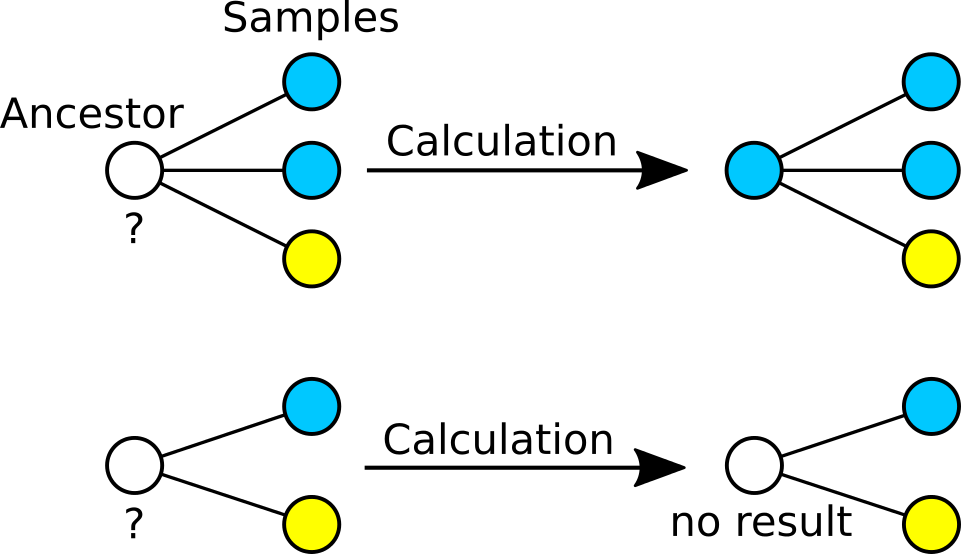
\includegraphics[width=8.14cm]{img/modal.png}
\caption{\label{modal} Calculation of an ancestor's mutational
value from a set of samples. The calculation is only possible
if we have at least three samples.}
\end{figure}

Because mutation rates are usually very slow we may assume
that a mutation occurs rarely. In this case the modal value
of a mutation is identical to the value that occurs most
often among the samples. The rare cases are the mutations.
If the time spans get very long this is no longer true. We
have no idea how many mutations have occurred between the
ancestral haplotype and the modern samples. The mutational
values are just random. If we use them to calculate the modal
haplotype, the result will be different from the real ancestral
values.

So for a valid calculation of a modal haplotype, two
conditions must be satisfied:

\begin{enumerate}
\item We must have at least three samples and two of them must
	have the same mutational value.
\item The time span between two ancestral haplotypes must be
	small compared to the average time in which a mutation occurs.
\end{enumerate}


\subsection{Maximum Parsimony Method}

As default Phyloage uses an algorithm that tries to satisfy
the maximum parsimony criterion \cite{Wiki-Maximum_parsimony}.
This means that the tree that contains the least amount of
mutations is considered best.

Although this is very intuitive and widely used, it is not
always true or easy to calculate because

\begin{enumerate}
\item In many cases there is no best tree, but a number of
	viable solutions. As an easy example consider two persons
	with two different values for the same marker. Both values
	are valid solutions for the modal haplotype.
\item Long time single lineages may introduce a set of completely
	random values, because it is likely that marker's have changed
	several times. The criterion of maximum parsimony can be
	misleading \cite{Fels78}.
\item The calculation of the most parsimonious tree can require
	enormous amounts of computing time \cite{Wiki-Maximum_parsimony}.
	In such cases we prefer a good solution over the best one possible.
\end{enumerate}

\begin{figure}[ht]
\centering
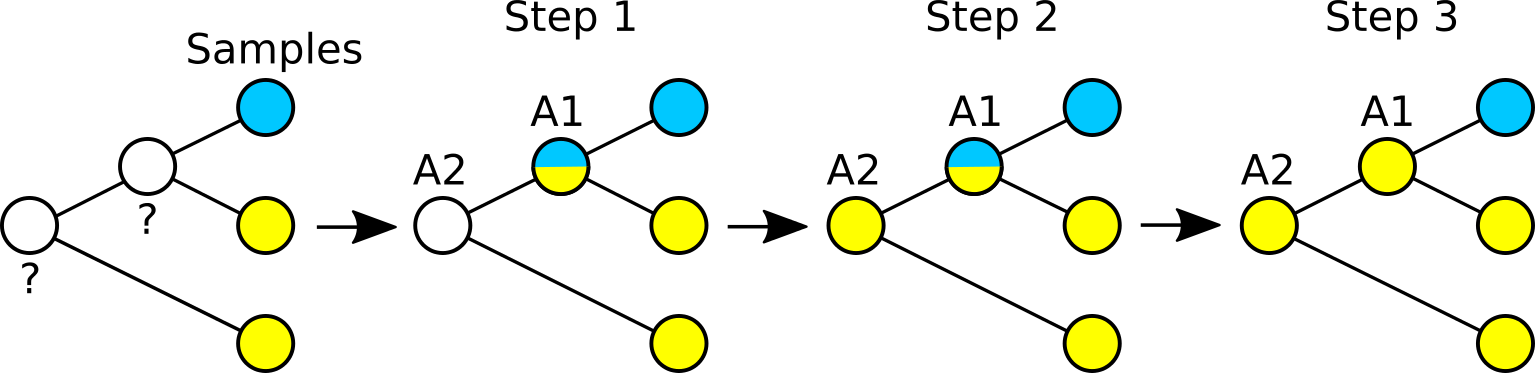
\includegraphics[width=13cm]{img/parsimony.png}
\caption{\label{parsimony} An algorithm that satisfies the
criterion of maximum parsimony. The tree is calculated backwards
until a unique modal value is found. After that the missing
values are recalculated.}
\end{figure}

Figure \ref{parsimony} shows how the most parsimonious solution
is derived for a very simple phylogenetic tree. In this 
example the modal values are calculated backwards in time until
a valid solution is found. After that the tree is recalculated
from the past to the present to find modal values for nodes that
did not have a viable solution before.

In reality the situation is more complicated because in many
cases there simply is no valid solution for a certain marker.
The algorithm that is used by Phyloage works like this:

\begin{enumerate}
\item If possible, modal values that strictly satisfy the
	maximum parsimony criterion are calculated. These are
	the easy cases.
\item The rest of the modal values are calculated by using
	averages and real numbers. This solution should come
	close to the maximum parsimony criterion, at least for
	many samples. In reality this solution is not possible
	because real marker values are restricted to whole numbers.
\item The modal values are mapped to their nearest neighbors
	from the set of real marker values. Still some markers
	can not be calculated because they do not have a unique
	nearest neighbor.
\item All markers that could not be calculated in the top
	node are forced to a real world neighbor value. After
	that the whole tree is recalculated and all markers are
	forced to a real world value.
\end{enumerate}

The algorithm does not necessarily find the best solution
possible, but it should find a good one. For more information
please consult the program's source code documentation
\cite{PhyloageSourceDoc} directly.


\subsection{Phylofriend Method}

Phyloage also provides an alternative method to calculate
the modal haplotypes. It is very simple and uses the same
algorithm as the Phylofriend \cite{Phylofriend} program.

\begin{figure}[ht]
\centering
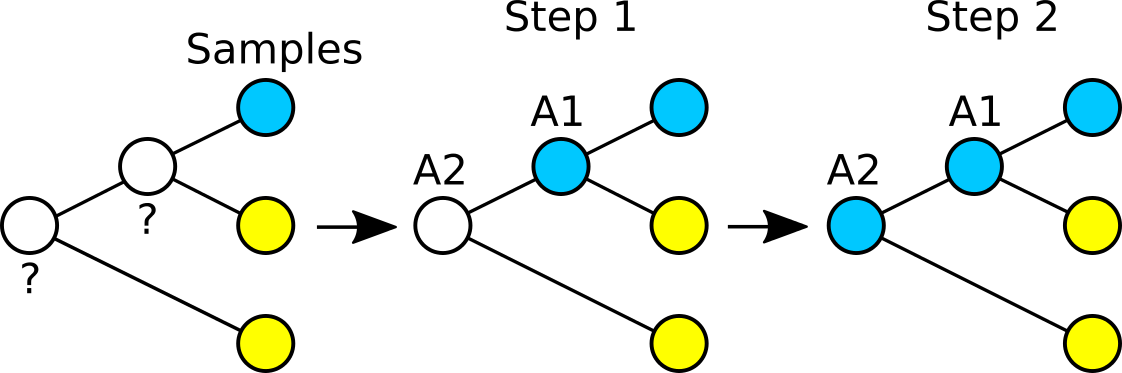
\includegraphics[width=9.5cm]{img/phylofriend.png}
\caption{\label{phylofriend} The Phylofriend method to
determine a modal haplotype is very simple. If a modal
value can't be calculated, it just guesses and continues
the calculation.}
\end{figure}

Figure \ref{phylofriend} illustrates how Phylofriend calculates
a modal haplotype. Generally it chooses the most common value
as the ancestral value. If there is no most common value it
just guesses among the valid ones. This works very well if
a modal haplotype has many samples (at least three) downstream
of it's own. For just two samples the resulting modal haplotype
will be somewhere in between the two sample haplotypes.

This algorithm does not satisfy the maximum parsimony criterion,
but for sparse trees it works better than some might expect.
The reason is that a modal haplotype, that is calculated only
from samples, can not be influenced by older modal values afterwards,
thus eliminating the effect of distant single lineages.

What method to use depends highly on tree structure and
research goals. I am afraid that I can not give a general
recommendation. For sparsely populated trees both methods won't
work very well due to the difficulties involved.
For densely populated trees both methods, maximum parsimony
and phylofriend, should yield similar results.





